\section{Performance of Gesture Recognition}\label{sec:gestureperformance}
Gesture recognition is a core part of our solution and it is being performed often. 
Since the gesture recognition is being performed by a device with somewhat low performance,
it is important that we have high performance of our gesture recognition. 
In this section we test the performance of recognizing gestures. 
We test the performance by gradually populating the database with gesture traces and see how fast we can recognize a random gesture input.
We expect the number of gesture traces in the database to increase the recognition time.

For this setup, we add five gesture traces at a time. 
This is to simulate training a gesture five times, 
as recommended by \cite{threedollar}. 
We then generate a random gesture input, 
and run the recognition function on it ten times, 
logging the execution time.
We repeat this until there is a total of \num{100} gesture traces in the database, 
which corresponds to \num{20} unique gestures.
We performed this test six times on an iPhone 5, 
with a \SI{1.3}{\giga\hertz} dual-core ARM processor and \SI{1}{\giga\byte} RAM, running iOS \num{9.1}.

\begin{figure}[!htb]
    \centering
    \begin{tikzpicture}
  \begin{axis}[
%      ybar,
%      bar width=2pt,
      xlabel = Number of unique gestures,
      ylabel = Average time in ms,
      xtick=data,
      width=0.95\textwidth,
      height = 6cm,
      yticklabel style={align=right,inner sep=0pt,xshift=-0.3em},
      enlargelimits = false,
      ymax = 150,
      grid=major,
      try min ticks=10]]
    \addplot table[x=gestureNo, y=time] {data/three-dollar-test-results/results/10xrecognize/average.csv};   
  \end{axis}
\end{tikzpicture}
    \caption{Graph showing the time of recognizing gestures, with increasing number of gesture traces. Each unique gesture is training \num{5} times.}
    \label{fig:performancegraph}
\end{figure}

During testing we noticed that the ``Three Dollar Gesture Recognizer'' used a high amount of memory. Furthermore it did not properly release this memory and as a result the app would terminate during tests if we ran them for too long.
\Cref{fig:threedollarmemory} shows the amount of memory used by our app in a timespan of one minute and thirteen seconds, starting at the point where the app was launched on the iPhone. 
The first dotted line shows the time when the test began and the second dotted line shows when the test was finished and ``\$3'' started cleaning up it's resources.
However, as the graph shows, the memory use stays high after cleanup.
This issue is the reason we only repeat recognition ten times for each gesture, as more would cause the app to shut down due to excessive memory usage.

\begin{tikzpicture}
    \centering
    \node[anchor=south west,inner sep=0] (image) at (0,0) {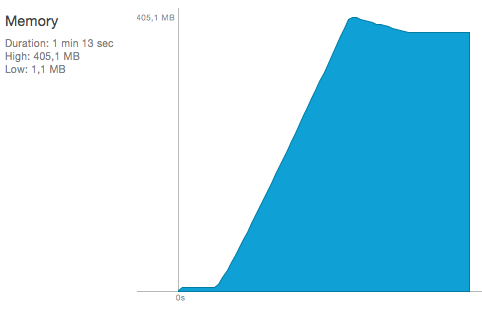
\includegraphics[width=0.7\textwidth]{images/three-dollar-memory-use.png}};
    \begin{scope}[x={(image.south east)},y={(image.north west)}]
        \draw[red,ultra thick, dotted] (0.45,0.08) -- (0.45,0.97);
        \draw[red,ultra thick, dotted] (0.73,0.08) -- (0.73,0.97);
    \end{scope}
\end{tikzpicture}

\subsection{Performance of Gesture Recognition Conclusion}
The result from \Cref{fig:performancegraph} shows that the time spent recognizing a gesture, 
increases linearly with the amount of gesture traces in the database.
As our system only attempts to recognize a gesture once, 
the performance of the ``Three Dollar Gesture Recognizer'' should be adequate for use in our system. 
The memory issues encountered during testing however showed that it might not be an appropriate solution if the system is to run for a prolonged period of time.
